\chapter{Experimental Setup}\label{experimental_setup}
	\section{Requirements}\label{requirements}
		In order to improve on previous works (cite Leonie, section \ref{related_work}), we require that our method fulfills following criteria:
	\begin{itemize}
		\item \textbf{R1: Minimal distance to water surface}: This requirement defined our experimental setup. As shown in figures \ref{fig:aquarium_setup} and \ref{fig:aelotron_setup}, lighting bubbles from below gives more freedom for the camera to be closer to the water surface. This is more apparent when the camera faces the surface with a certain angle. 
		\item \textbf{R2: Consistent image results}: Bubbles can look very different under different lighting conditions. For instance, bubbles might appear as dark disks or bright rings (chapter \ref{related_work}) depending how they are lit. We therefore require that the angle between camera and light source is always constant. This requirement guarantees a consistent pattern for bubbles across different water tanks.
		\item \textbf{R3: Images must contain all possibly retrievable information}. From our simulation (figure \ref{subfig:bubble_simulation}) we know that bubbles are characterized by two peaks. Both of these – especially the upper, dimmer one – are required to be visible. This requires the camera to have a high signal-to-noise ratio and/or the light source to be very bright. 
	\end{itemize}	
		
	\section{Aquarium Setup}
		\begin{figure}
			\centering
			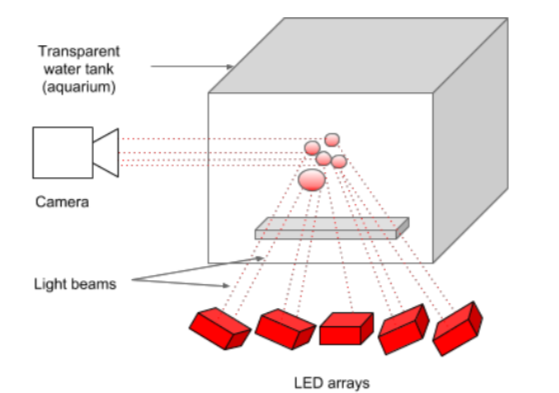
\includegraphics[scale=1]{images/aquarium_setup}
			\caption{Experimental setup illustrating the $90^\circ$ angle between the light source (LED array) and the camera. Note how LEDs are also oriented towards the camera's field of view to maximize the amount of light reaching the camera and therefore reduce noise.}
			\label{fig:aquarium_setup}
		\end{figure}			
		
		The goal of this setup is to capture bubble images that can be used to prototype our algorithm, so we built the experiment in a transparent $1m \times 1m \times 1m$ water tank as shown in figure \ref{fig:aquarium_setup} where we could change most of the parameters such as lighting angle, camera and bubble concentration independently from each other. Measurement results are discussed in next chapter and image analysis is discussed in chapter \ref{the_algorithm}.
		
		In order to satisfy requirements in section \ref{requirements}, we opted for the following parameters (also summarized in table \ref{tab:aquarium_param})
		
		\begin{itemize}
		\item \textbf{Camera} We chose the Basler A1920 mainly because of its high signal-to-noise ratio, and therefore fulfilling requirement R3 given enough light. Its main drawback is its relatively low frame rate at the highest possible resolution, which making bubble tracking more difficult, which in turn makes radius calibration more difficult (see section \ref{calibration_setup}. Compared to an available high-speed camera with comparable maximum resolution, (PCO Dimax, 1,2kHz at $2000 \times 2000$ resolution) our chosen camera also has a smaller sensor. This means that the magnification factor is higher and therefore smaller bubbles can be better detected as well. 
		
		\item \textbf{Lens} A 100 mm macro lens was used in this setup. The large focal length yields a large magnification, which is desired.
		\item \textbf{Exposure time} This value depends on the maximum speed of bubbles. In this setup, no waves are present, so a bubble's speed is proportional to its radius. 
		\item \textbf{F-number} This value has been chosen such that the depth of field is a few centimeters large (see also section \ref{calibration_setup})		
		\item \textbf{Air flow} Bubbles were produced by an bubble generator. Bubble radii therefore depend on the amount of air flowing through the bubble generator (measured in liter per minute or LPM).
		\end{itemize}
		
		\begin{table}
			\centering
		
			\begin{tabular}{|c|c|}
			\hline 
			Camera & Basler A1920-155um \\ 
			\hline 
			Focal length & 100 mm \\ 
			\hline 
			F-number & 5,6 \\ 
			\hline 
			Exposure time & 100 us \\ 
			\hline 
			Resolution [px] &1920 x 1200 \\
			\hline 
			Sensor size & 11.3 mm x 7.1 mm \\
			\hline
			Air flow & 1,8 LPM \\ 
			\hline 
			Magnification factor & 30 um/px \\ 
			\hline 
			Framerate & 100 Hz \\ 
			\hline 
			Resulting field of view & 5,7cm x 3,6 cm \\
			\hline
			\end{tabular} 
			
			\caption{Parameters for aquarium setup}
			\label{tab:aquarium_param}

		\end{table}
		
	\section{Aeolotron Setup}
		The Aeolotron is an experimental annular wind-wave facility with a diameter of about 10m and a width of about 60cm. Typical water height is 1m. Four wind engines generate reference wind speeds of up to 14m/s, enough to generate breaking waves that in turn produce air bubbles. Figure \ref{fig:aeolotron_setup} shows a schematic view of the wind facility as well as the experimental setup.
		
		The goal of this setup is to apply the knowledge gained from the previous setup on bubble measurements emerging from breaking waves, so we reproduced the setup from the aquarium at the Aeolotron, while keeping as many unchanged parameters as possible (e.g. same camera, same light source same lens etc...). 
		
	We also used a bubble generator first, to verify that the algorithm developed for the previous setup still works with measurements from the Aeolotron setup. Some parameters such as focus distance and angle between the light source and bubbles were inevitably changed, which means we needed to calibrate the depth of field again. 
		
		\begin{figure}
			\centering
			\begin{subfigure}[b]{.55\textwidth}
				\centering
				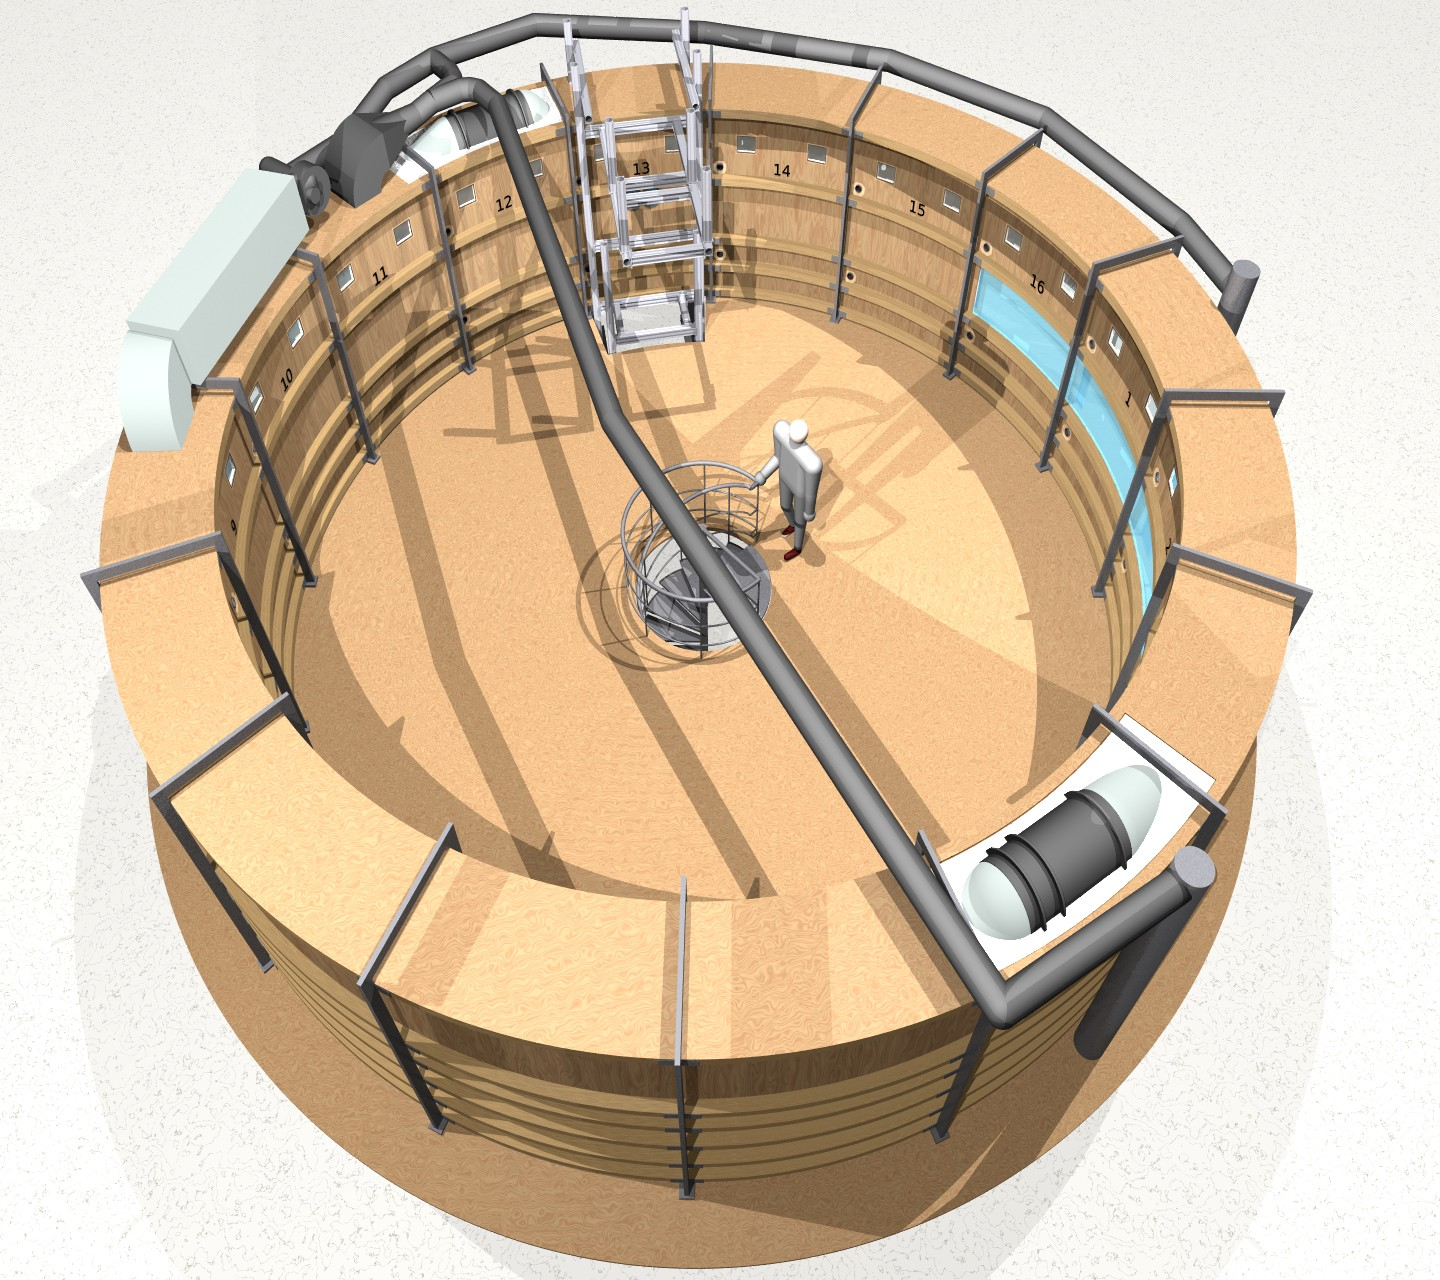
\includegraphics[scale=0.1]{images/aeolotron-gesamt.jpg}
				\caption{Aeolotron wind wave facility}
			\end{subfigure}

			\begin{subfigure}[b]{.55\textwidth}		
				\centering
				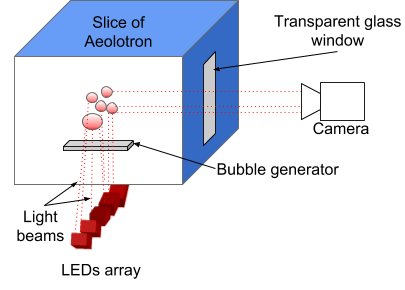
\includegraphics[scale=.8]{images/aeolotron_setup.png}
				\caption{Experimental setup}
			\end{subfigure}
			
			\caption{Aeolotron facility and experimental setup}
			\label{fig:aeolotron_setup}
		\end{figure}
	
		
		
	\section{Measurement result}\label{measurement_result}
	\section{Calibration}\label{calibration_setup}


































